\section{Měření kondenzátorů}
Měření hodnot kapacity se stává samostatnou částí a provádí se měřením doby nabíjení.\\
Původní software Markuse F. to dělal pomocí programové smyčky, která četla příslušný digitální
vstupní pin až do doby změny signálu a přitom sčítala průchod smyček.\\
To má tu nevýhodu, že je rozlišení časového měření omezeno celkovým časem průchodu smyčkou.\\
Toto bylo obvykle provedeno ve všech šesti možných kombinacích tři zkušebních pinů.\\
Současný software používá dva různé způsoby, jak přečíst pouze tři
možné kombinace pro tři zkušební kolíky.\\
Pozitivní stranou je nyní vždy vyšší číslo zkušebního pinu.\\
Pouze pokud je kapacita měřena společně s paralelně zapojenou diodou,
může mít polarita jiný směr.

\subsection{Vybíjení kondenzátorů}
Vždy byste měli kondenzátor vybít dříve, než bude připojen k testeru.\\
Před zahájením jakéhokoliv testu bude kondenzátor přesto ještě jednou testerem vybit.\\
Je-li napětí nižší než \(1300mV\) ,  bude kondenzátor na připojeném ADC portu (Port C) zkratován.\\
Myslím, že je to v pořádku, protože každý portový výstup má vnitřní odpor asi \(20\Omega\).\\
Obrázek 149 (strana 258) v datovém listu ATmega8 \cite{ATmega8} ukazuje pokles napětí výstupních pinů, až na hodnotu \(2V\). Samozřejmě, nelze zaručit, že se nenastane žádná škoda.\\
Testoval jsem tuto funkci velmi často s kondenzátory většími než \(15mF\)  a nikdy jsem si nevšiml nějakého problému.\\
Proud by měl zůstat pod stanovenou mezní hodnotou \(40mA\) a bude rychle vybíjením redukován.\\
Samozřejmě může dojít k poškození, pokud (vysokonapěťový) kondenzátor před připojením k testeru, úplně nevybijete.
\subsection{Měření velkých kapacit}
\label{sec:bigcap}
Jedna strana kondenzátoru je připojena k GND.\\
Druhá strana je, pomocí \(680\Omega\) odporu, připojena k VCC na dobu \(10ms\).\\
Pak se tento měřicí kolík přepne na vstup (vysoká impedance).\\
Po tomto proudovém impulzu se napětí na kondenzátoru měří bez proudu.

Pokud napětí nedosáhlo minimální hodnoty \(300mV\), opakuje se tento nabíjecí impuls dalších 499krát.\\
Když po 127 pulsech (přibližně \(2s\)) nebylo dosaženo minimálního napětí \(75mV\), proces nabíjení bude přerušen, protože se zbývajícími nabíjecími impulzy nebude \(300mV\) dosaženo.

Obrázek~\ref{fig:bigcap1} ukazuje tři fáze určení kapacity kondenzátoru.\\
Hodnota kapacity se pak vypočte z počtu nabíjecích impulsů a dosaženého nabíjecího napětí pomocí tabulky.\\
Tabulka obsahuje, při rozsahu napětí \(25mV\), faktory pro výpočet, z doby nabíjení a napětí, hodnoty kapacity.

Mezi-produktové hodnoty napětí jsou interpolovány.

\begin{figure}[H]
\centering
 \begin{overpic}[width=16cm]{../FIG/Bigcap.pdf}
  \color{black}
  \put(25,97){\makebox(0,0)[cb]{rychlé vybíjení kondenzátoru}}  
  \put(25,61){\makebox(0,0)[cb]{10ms fáze nabíjení kondenzátoru}} 
  \put(25,26){\makebox(0,0)[cb]{měřící fáze nabíjení kondenzátoru}}      
 \end{overpic}
\caption{Vybíjení a nabíjení kondenzátoru s \(10ms\)  nabíjecími impulzy na napětí \textgreater~\(300mV\)}
\label{fig:bigcap1}
\end{figure}

Vzhledem k nízkému nabíjecímu napětí se měření stává mnohem rychlejší než u původní verze softwaru,
protože tato výhoda funguje také při vybíjení. To umožňuje měřit větší kondenzátory.\\
Kromě toho ve většině případů nezasahuje paralelní dioda do měření, protože nebude dosaženo její prahové napětí.

Po verzi 1.12k softwaru byl použit trik pro zjištění zbytkového napětí kondenzátoru ještě před měřením. Zbytkové napětí může být kladné nebo záporné v závislosti na historii.
ADC však nemůže měřit záporné napětí. Proto je napětí záporného zkušebního pinu s \(680\Omega\) odporem zvýšeno na přibližně \(132mV\), jak ukazuje obrázek~\ref{fig:CapResidV}.
Zbytkové napětí může být nyní tvořeno, z rozdílu napětí, na obou stranách kondenzátoru. Napětí na kladném zkušebním pinu zůstává v každém případě pozitivní, i když kondenzátor má záporné zbytkové napětí několika mV.

\begin{figure}[H]
\centering
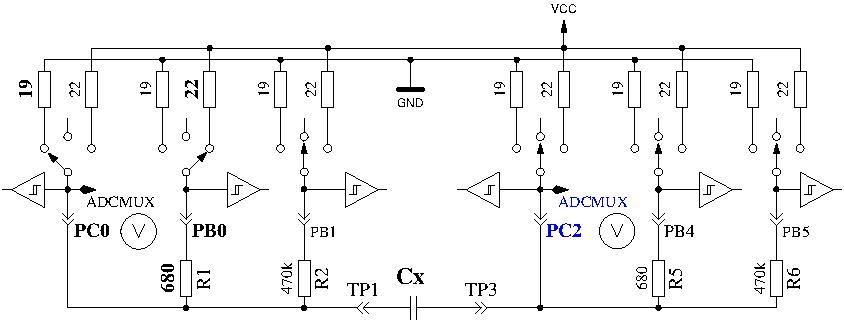
\includegraphics[]{../FIG/Cap_residV.pdf}
\caption{Měření zbytkového napětí kondenzátoru při počátku nabíjení}
\label{fig:CapResidV}
\end{figure}

Obrázek~\ref{pic:c229} ukazuje nabíjení a vybíjení velkého kondenzátoru \(229\mu F\).\\
Plochá střecha měřicí křivky až do začátku vybíjení je způsobena časem měření a dobou výpočtu ATmega.\\
Obrázek~\ref{pic:c5mF} ukazuje stejné měření pomocí kondenzátoru~\(5mF\),
Všimněte si, jak se doba měření včetně vybíjení zvýšila na přibližně 1,5 sekundy.\\
\begin{figure}[H]
  \begin{subfigure}[b]{9cm}
    \centering
    \includegraphics[width=9cm]{../PNG/charge_229uF.png}
    \caption{\(229\mu F\)-Kondenzátor}
    \label{pic:c229}
  \end{subfigure}
  ~
  \begin{subfigure}[b]{9cm}
    \centering
    \includegraphics[width=9cm]{../PNG/charge_5mF.png}
    \caption{\(5mF\)-Kondenzátor}
    \label{pic:c5mF}
  \end{subfigure}
  \caption{Nabíjení a vybíjení velkých kondenzátorů pro měření}
\end{figure}
Poslední příklad na obrázku~\ref{pic:c15mF} ukazuje měření kondenzátoru \(15mF\).
\begin{figure}[H]
  \centering
    \includegraphics[]{../PNG/charge_15mF.png}
  \caption{Nabíjení a vybíjení \(15mF\) kondenzátoru pro měření}
  \label{pic:c15mF}
\end{figure}

Po tomto měření kondenzátoru bude zkoumáno samovybíjení kondenzátoru pomocí
zkoušky ztráty napětí v úměrném čase době nabíjení.\\
Naměřená kapacitní hodnota kapacity je odpovídajícím způsobem upravena.\\ Test \(68\mu F\) kondenzátoru s paralelně zapojeným \(2,2k\Omega\) odporem ukazuje účinnost této metody.

Zjištěná hodnota kapacity bez odporu
je \(66,5\mu F\), s paralelním odporem \(2,2k\Omega\) je měřena hodnota kapacity \(65,3\mu F\).\\
Pro srovnání bych rád specifikoval odpovídající výsledky s Peaktech 3315 multimetrem.\\
Bez odporu se měří kapacita \(68,2\mu F\), s paralelním \(2,2k\Omega\) odporem je však, pomocí multimetru, naměřeno \(192\mu F\)  .

\subsection{Měření malých kapacit}
Pokud první \(10ms\) nabíjecí impuls přetížil kondenzátor, je použita jiná měřicí technika.

Mikrokontrolér ATmega má vestavěný 16bitový čítač, který to zvládne při maximální taktové frekvenci (\(1MHz\) nebo \(8MHz\)).\\
Tento čítač má také schopnost, kvůli externí události, uložit svoji momentální hodnotu do paměti.

Tato hodnota může být také výstupní signál komparátoru.\\
Komparátor může pracovat s libovolným vstupním kolíkem ADC a referenčním napětím (Band Gap Reference).

Schéma zapojení~\ref{fig:comparat} ukazuje zjednodušený diagram situace měření.\\
Takže vybijí kondenzátor, připravím komparátor pro správný pin vstupu, vynuluji počítadlo a začnu okamžitě nabíjet kondenzátor.
Jedna strana kondenzátoru je připojena k GND, druhá strana přes \(470k\Omega\) odpor k VCC.\\
Nyní zkontroluji programovou smyčkou, zda počitadlo hlásí přeplnění (overflow) nebo externí událost (input capture).
Sčítám tak dlouho události přeplnění, pokud nezjistím externí událost.

V takovém případě zastavím čítač a kontroluji, zda musím ještě jedno další přetečení přičíst,
protože čítač nelze, pomocí externího vstupu (input capture), zastavit.

Sčítání externí události s počítadlem přetečení, tvoří celkový čas, z kterého je s faktorem kapacita určena.
Současný software může tabulku s teoretickou závislostí doby načítání ve vztahu k naměřené 
hodnotě srovnávacího napětí porovnat.\\
Tabulka obsahuje hodnoty ve stupních \(50mV\), výsledky jsou interpolovány podle aktuálního referenčního napětí.
Tato tabulka je aktivována pouze volbou Makefile WITH\_AUTO\_REF.

Z hodnoty kapacity preferuji experimentálně zjištěnou předdefinovanou konstantu nebo jednu v autotestu
zjištěnou konstantu pro odstranění ofsetu naměřené hodnoty.
Nevím, jestli má být předdefinovaná konstanta upravena pro jiné varianty testeru.
Při autotestu s nastavením možnosti AUTO\_CAL-Option se toto nastavení provede automaticky.

Všiml jsem si, že referenční napětí je obvykle příliš malé, proto můžete zadat doplněk s 
volbou Makefile REF\_C\_KORR.
Po kalibraci s volbou AUTO\_CAL-Option je hodnota REF\_C\_KORR-Wert jen korekce k automaticky
zjištěnému rozdílu mezi nabitým kondenzátorem a vnitřnímu referenčnímu napětí.\\
Naměřené referenční napětí se pak koriguje (přidává) s hodnotou (v mV).
Pokud není použita volba WITH\_AUTO\_REF bude referenční napětí stejné jako v
dokumentech ATega8, ATmega168 a ATmega328 viz dokumentace ~\cite{ATmega8}~\cite{ATmega168}.
Příklad měření tohoto typu je zobrazeno na obrázku~\ref{pic:c22uF}.
Doba měření pro kondenzátor \(22\mu F\)  je přibližně \(2,6s\) protože \(470k\Omega\) odpor se používá k nabíjení.
V tomto případě je však vybíjení mnohem rychlejší než nabíjení.

\begin{figure}[H]
\centering
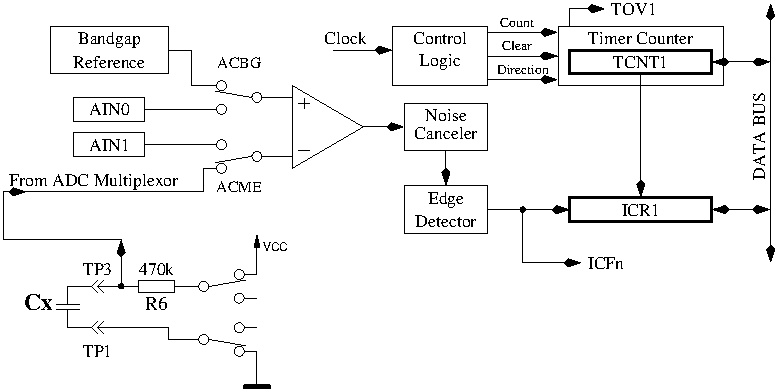
\includegraphics[]{../FIG/Comparat.pdf}
\caption{Měření malých kapacitních hodnot s komparátorem}
\label{fig:comparat}
\end{figure}

\begin{figure}[H]
  \centering
    \includegraphics[]{../PNG/charge_22uF.png}
  \caption{Nabíjení a vybíjení \(22\mu F\) kondenzátoru pro měření}
  \label{pic:c22uF}
\end{figure}


V zásadě lze tuto techniku použít také s \(680\Omega\) odporem,
ale protože ADC nemůže být používáno během provozu komparátoru, neexistuje žádná
možnost sledování nabíjecího napětí až do zastavení komparátoru.

Je-li neznámá dioda spojena paralelně s kondenzátorem, může být nabíjecí proud
absorbovat diodou (prahové napětí) a referenční napětí by nikdy nebylo dosaženo.
Této koncepční chybě se zabraňuje metodou popsanou v současném softwaru pro velké kondenzátory
v kapitole~\ref{sec:bigcap}.

\subsection{Měření velmi malých kapacit metodou vzorkování}
Amatérský radiový operátor Pieter-Tjerk (PA3FWM) rozšířil schopnosti testeru o měření velmi malých kapacit (\textless~100pF) s vysokým rozlišením metodou vzorkování ADC.\\
Doba konverze ADC není vlastně dostačující, aby bylo možné skenovat rychlé procesy.\\
Při odběru vzorků napětí je zde však vstupní signál vzorkován v přesně stanoveném čase,
době vzorkování(sample) a přidržení (hold) = (SH).\\ ADC potřebuje pro úplnou konverzi 13 taktů,
přičemž je tento takt získán dělením procesorového taktu 128 nebo 64.
Vzorkování hodnoty napětí vždy probíhá přesně na cyklu ADC 1.5.\\
Pokud je nyní možné, skenovat velikost napětí a stále znovu vytvářet, pak je také možné,
posunem času vzorkování odebrat, pomocí rastru ofsetu, kompletní signál.

Normální konverze ADC trvá na \(8MHz\) procesorových taktů 13x64 = 832 taktových cyklů.\\ 
Pokud se nyní signál s cyklem 831 taktů opakuje, bude nepřerušená konverze ADC (režim volnoběhu) tohoto
signálu, je při každé konverzi, jeden procesorový takt později odebrán.\\
Při této metodě je třeba dbát na to, aby start první konverze ADC signálu  začal v požadovaném času\\.
Doba následných hodnot ADC se posune vždy o jeden takt procesoru relativně k nově generovanému signálu.\\
Pokud je opakování impulsu úspěšné, odpovídá pak hodnota složena z mnoha opakování impulsu, ADC signálu,
který je vzorkován a převeden s \((8MHz\)) procesorovým taktem .

Obrázek~\ref{fig:sampling} ukazuje princip odběru vzorků desetkrát opakovaných impulsů k získání 10 vzorků (SH0 - SH9).\\
Pro reálný případ je relativní časový posun postupných vzorků mnohem nižší, než je zobrazeno.

\begin{figure}[H]
\centering
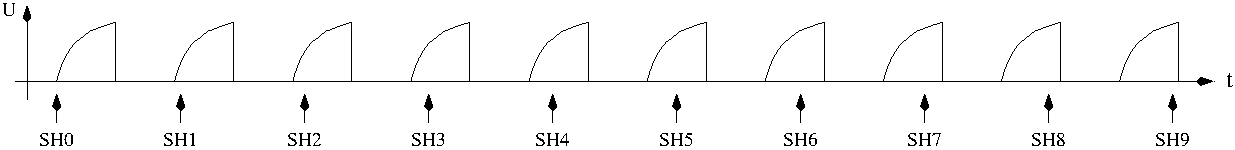
\includegraphics[width=18cm]{../FIG/sampling.pdf}
\caption{Odběr průběhu napětí metodou vzorkování}
\label{fig:sampling}
\end{figure}

Obtížnost pro přesné stanovení prvního vzorkovacího času vyplývá ze skutečnosti, že
oddělovač pro generování taktu ADC může být restartován pouze s externím signálem.\\
Při spouštění ADC z programu  čítač nepřestane počítat.

Soulad s přesným počátečním a časovým obdobím je možný pouze v strojovém jazyce (assembler),
protože zde závisí na každém taktu procesoru.

Při odběru vzorkovací křivky malých kondenzátorů pomocí metody vzorkování se ukázalo,
že časová konstanta nezůstává, během doby vzorkování, konstantní. To Pieter-Tjerk v jedné
prezentaci na 60. konferenci VHF ve Weinheimu (D) představil.

Asi \(10pF\) kondenzátor, který drží napětí pro konverzi ADC, je v SH čase pro konverzi odpojen a asi dva ADC takty později znovu připojen.\\
Kromě toho je tam, půl ADC taktu předem, ještě malá nepravidelnost v datech, která je pravděpodobně
způsobena přepnutím multiplexeru.\\ Obě poruchy jsou zohledněny v softwaru.\\
Software pro odběr vzorků může digitalizovat 255 hodnot, přičemž pro vzorkování nabíjecí křivky lze
také použít výpočet průměrů 32 digitálně.\\ Tím je možné vliv poruchy mírně snížit.
Software dokáže měřit jak proces nabíjení, tak i vybíjení.

Protože při měření kapacity usměrňovací diody jsou měřeny oba procesy,
je kalibrace nulové kapacity provedena v obou směrech a při všech kombinacích měřících pinů.

Měřením kapacit během procesu nabíjení a vybíjení může být zobrazena závislost kapacity spojení na napětí, protože je nabíjecí kapacita měřena kolem 0V a proces vybíjení je měřen téměř u 5V.
Normální kondenzátor by neměl, při tak nízkém napětí, žádný rozdíl kapacity ukázat.\\ Zde je tedy kapacita měřena pouze během nabíjení.

Pieter-Tjerk optimalizoval funkci pro provoz \(16MHz\). Zde je dosaženo rozlišení \(0,01pF\).\\
Při provozu s \(8MHz\) běží převodník ADC pro vzorkovací metodu s poloviční frekvencí, aby hodnota
dříve zmíněných rušivých vlivů ležela na stejných datových pozicích.\\
Ztráta rozlišovací schopnosti, v důsledku použití \(8MHz\) krystalu, nehraje většinou žádnou roli
a také doba měření zůstává v tolerovatelnějších mezích.

\subsection{Měření ekvivalentního sériového odporu ESR}

ESR \cite{ESR}  je měřítkem stárnutí elektrolytických kondenzátorů.\\

Obrázek~\ref{fig:Cap_equiv} ukazuje ekvivalentní obvod kondenzátoru.

Odpor \(Rp\) představuje izolační odpor kondenzátoru,

odpor \(ESR\) představuje ekvivalentní sériový odpor

a \(ESL\) ekvivalentní sériovou indukčnost.

\begin{figure}[H]
  \centering
    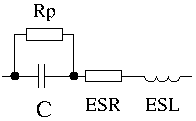
\includegraphics[]{../FIG/Cap_equiv.pdf}
  \caption{Ekvivalentní obvod kondenzátoru}
  \label{fig:Cap_equiv}
\end{figure}

V datových listech je běžné, udávat ESR při frekvenci \(100kHz\) a teplotě \(20\textdegree C\).\\
Obrázky \ref{fig:Cap_FC_data} a \ref{fig:Cap_FR_data} ukazují výrobcem Panasonic
specifikované  \(ESR\) hodnoty pro elektrolytické kondenzátory při různých provozních napětí pro FC 
a ,,low ESR'' série. \\
Obě série jsou určeny pro maximální teplotu \(105\textdegree C\).

Obrázek \ref{fig:Cap_FC_FR_data} představuje předepsaná data obou sérií při přípustném provozním napětí \(25V\). Pokud jsou v sérii k dispozici různé modely se stejnou kapacitou a napětím,
jsou zobrazena data s nejnižším \(ESR\).\\
U elektrolytických kondenzátorů je ESR a kapacita relativně silně závislá na provozní teplotě.

\begin{figure}[H]
  \centering
  \includegraphics[width=14cm]{../GNU/Cap_FC_dataCZ.pdf}
  \caption{ESR hodnoty z datového listu Panasonic série FC}
  \label{fig:Cap_FC_data}
\end{figure}

\begin{figure}[H]
  \centering
  \includegraphics[width=14cm]{../GNU/Cap_FR_dataCZ.pdf}
  \caption{ESR hodnoty z datového listu Panasonic série FR}
  \label{fig:Cap_FR_data}
\end{figure}

\begin{figure}[H]
  \centering
  \includegraphics[width=14cm]{../GNU/Cap_FC_FR_dataCZ.pdf}
  \caption{Porovnání ESR hodnot série FC a FR}
  \label{fig:Cap_FC_FR_data}
\end{figure}

Měření při \(100kHz\) není s hardwarem ATmega snadné, protože ani ADC neumožňuje při takové vysoké vstupní frekvenci přímé vzorkování, ani není \(100kHz\) signál ve stávajícím okruhu k dispozici.

Následovně budou prezentovány dvě metody pro určení  \(ESR\), které jsou s existujícím okruhem možné.\\
Obě metody používají  pro měření pravoúhlý měřicí signál, takže výsledky nikdy nemohou přesně odpovídat údajům, měřeným sinusovým signálem.
V první metodě jsou výsledky blízké   \(ESR\) hodnotám získaným u \(1kHz\).

Nicméně má druhá metoda výhodu, že se zkratovanými zkušebními piny, může být nastavena nula a dále, že zjištěná  \(ESR\) se blíží hodnotě, naměřené při \(10kHz\).
V současné době nemám nápad na metodu měření, která může poskytnout srovnatelnou ESR hodnotu, jako \(100kHz\)  měření.
Následující tabulka \ref{tab:capESR} by měla ukázat závislost \(ESR\) na frekvenci.
S výjimkou kondenzátoru \(47\mu F\) jsou všechny kondenzátory z řady Panasonic FC.
Referenční hodnoty byly stanoveny měřidlem Peaktech 2170 LCR.
Všechny výsledky testeru v této tabulce byly porovnány s výsledky v podkapitole \ref{sec:ESR2} popisované metodě 2.
U velkých kapacitních hodnot činí indukčnost \(ESL\), která je také přítomná, je měření,
při vyšších frekvencích \(100kHz\), velmy obtížné.


\begin{table}[H]
  \begin{center}
    \begin{tabular}{| l | c | c | c | c | c |}
   \hline
            & Datový list & PeakTech  & Peaktech & PeakTech & tester \\
Kondenzátor & 100 kHz    & 100 kHz   & 10 kHz   & 1 kHz    &   \\
    \hline
    \hline
1uF / 50V    & 2.4       & 1.27      & 1.75     & 4.31     &  2.1 \\
    \hline
2.2uF / 50V  & 1.8       & 1.07      & 1.34     & 2.76     &  1.6 \\
    \hline
4.7uF / 50V  & 1.3       & 1.19      & 1.40     & 2.37     &  1.5 \\
    \hline
4.7uF / 50V  & 1.3       & 1.19      & 1.40     & 2.37     &  1.5 \\
    \hline
10uF / 50V   & 1.3       & 1.26      & 1.45     & 2.05     &  1.5 \\
    \hline
22uF / 10V   & 2.0       & 1.52      & 1.76     & 2.24     &  1.9 \\
    \hline
47uF / 63V   & ?         & 0.46      & 0.50     & 0.63     &  0.52 \\
    \hline
    \end{tabular}
  \end{center}
  \caption{ESR hodnoty různých elektrolytických kondenzátorů}
  \label{tab:capESR} 
\end{table}


\subsection{Měření ekvivalentního sériového odporu ESR, metoda 1}
U kondenzátorů s více než \(0,45\mu F\) se pokouší měřit sériový odpor kondenzátorů.\\
Při více než \(3,6\mu F\) se pro převodník analogově-digitálního signálu používá normální taktová frekvence \(125kHz\).

Při menších kapacitách se urychluje měření pomocí zvýšené frekvence \(500kHz\).\\
Přesnost ADC výsledků bude při vyšší frekvenci sice horší, ale větší \(ESR\) hodnoty 
menší kondenzátory snižují vliv této ztráty přesnosti.\\
Na druhou stranu není možné měřit \(ESR\) pro kondenzátory pod \(1,8\mu F\) jinak pomocí této metody.

Přísně řečeno, závisí \(ESR\) kondenzátoru na provozní frekvenci a teplotě.
Obvykle je v datových listech uvedena hodnota naměřená sinusovým signálem při \(100kHz\).
Při této frekvenci nemůže ATmega, bez vnějších obvodů, měřit.

Níže popsaný postup dosahuje, při normální ADC frekvenci, pouze měřicí frekvenci pod \(640Hz\), s přibližně pravoúhlým signálem.\\ Při \(500 kHz\) ADC taktu se dosáhne frekvence měření přibližně \(2400Hz\).

Pro určení ekvivalentního sériového odporu, bude kondenzátor nejprve v jednom směru nabíjen a na obou svorkách jeho napětí s interním referenčním napětím (\(1,1V\)) měřeno.

Po měření se vypne nabíjecí proud a bude nyní měřeno napětí na kondenzátoru bez nabíjecího proudu.

Když je napětí na kondenzátoru bez nabíjecího proudu menší než \(3mV\) , bude tato sekvence měření opakována.

Obrázek~\ref{fig:Cap_esr} zobrazuje odpovídající obvody.

\begin{figure}[H]
  \centering
  \begin{overpic}[width=17cm]{../FIG/Cap_esr.pdf}
  \color{black}  
  \put(28,85){\makebox(0,0)[cb]{měření napětí s nabíjecím proudem}} 
  \put(28,40){\makebox(0,0)[cb]{měření napětí bez proudu}}      
  \end{overpic}
  \caption{Schéma ESR měření kondenzátoru}
  \label{fig:Cap_esr}
\end{figure}

Rozdíl napětí mezi kondenzátorem a proudem je měřítkem vnitřního odporu kondenzátoru.\\
Očekávaný rozdíl napětí je však tak malý, že s jedním měřením nelze dosáhnout žádného užitečného výsledku.

Z tohoto důvodu se proud převrací a měření se opakuje v opačném směru.\\
Celá sekvence měření je  128 krát opakovaná a výsledky měření napětí jsou sečteny.

Pak máte tři součty napětí, \(Ulp\) napětí na záporném pólu kondenzátoru s proudem, \(Uhp\) napětí na
pozitivním pólu kondenzátoru s proudem a \(Uc\) napětí na kladném pólu kondenzátoru bez proudu.

Součet napětí u záporného pólu kondenzátoru představuje pokles napětí v prostředním nabíjecím proudem při výstupním odporu portu \(Rport\).

Z rozdílu mezi součtem napětí na kladném pólu a záporným pólu kondenzátoru
lze dosáhnout míru napětí na kondenzátoru s nabíjecím proudem \(Udiff = Uhp - Ulp\).

Rozdíl \(Uesr = Udiff - Uc\) by nyní měl representovat pokles napětí u středního nabíjecího proudu na vnitřním odporu kondenzátoru.

Hodnota odporu bude zmenšena poměrem tohoto napětí \(Uesr\) k napětí \(Ulp\) známé hodnoty odporu výstupu
portu \(Rport\).

To zmenšení bude takové, aby bylo dosaženo rozlišení \(0,01 \Omega\) 
 \(Resr = \frac{Uesr \cdot 10 \cdot Rport}{Ulp}\).\\
Obrázek~\ref{pic:esr4} ukazuje část profilu napětí na \(4,2\mu F\) kondenzátoru během \(ESR\) měření.
 
K objasnění \(ESR\) vlivu byl Kondenzátor sériově propojen s \(6,8 \Omega\) odporem.\\ 
Malé napětí po skončení nabíjení kondenzátoru je vyhodnocováno softwarem.

Větší pokles napětí při měření proti GND je způsoben vlivem výstupního portu odpor asi \(20\Omega\).\\
Výsledkem \(ESR\) měření je tomto případě \(7,5 \Omega\), bez \(6,8 \Omega\) odporu to je \(0,56\Omega\).\\
Na obrázku~\ref{pic:esr2} ukazuje stejné měření s vyšší frekvencí měření v \(2,2\mu F\)
Elko s ESR \(6.5\Omega\).


\begin{figure}[H]
  \begin{subfigure}[b]{9cm}
    \centering
    \includegraphics[width=9cm]{../PNG/ESR_4uF.png}
    \caption{Pin naměřený proti GND}
  \end{subfigure}
  ~
  \begin{subfigure}[b]{9cm}
    \centering
    \includegraphics[width=9cm]{../PNG/ESR4uF6R8.png}
    \caption{Měřeno od pinu k pinu}
  \end{subfigure}
  \caption{Napěťová křivka \(4,2\mu F\) kondenzátoru během ESR měření}
  \label{pic:esr4}
\end{figure}

\begin{figure}[H]
  \begin{subfigure}[b]{9cm}
    \centering
    \includegraphics[width=9cm]{../PNG/ESR_2uF_pin2GND.png}
    \caption{Pin naměřený proti GND}
  \end{subfigure}
  ~
  \begin{subfigure}[b]{9cm}
    \centering
    \includegraphics[width=9cm]{../PNG/ESR_2uF_pin2pin.png}
    \caption{Měřeno od pinu k pinu}
  \end{subfigure}
  \caption{Napěťová křivka \(2,2\mu F\)  kondenzátoru během ESR měření}
  \label{pic:esr2}
\end{figure}

Přesnost ESR měření není z několika důvodů příliš vysoká:
\begin{enumerate}
\item Měření napětí na dvou koncích kondenzátoru nelze provádět současně, ale pouze po sobě.
 Mezitím se nabíjecí proud změnil v důsledku nabíjení kondenzátoru.
To se pokouší kompenzovat s kapacitní závislostí korekce napětí záporného pólu.
\item  ADC vezme hodnotu napětí 1,5 taktu po startu procesu konverze. Tato začíná stoupajícím bokem ADC taktu, když je nastaven počáteční bit. Pokud je nabíjecí proud kondenzátoru příliš brzy vypnutý,
přebírá ADC špatné napětí pro proudové měření. Pokud je nabíjecí proud vypnutý příliš pozdě, je kondenzátor 
déle nabíjený, než odpovídá měření proudu. Potom se v bezproudovém stavu měřeno příliš vysoké napětí.
V programu je však obtížné nastavit přesný čas vypnutí napájení.
\item Výstup odporu portu se používá jako referenční hodnota pro tuto měřicí metodu, tato hodnota odporu
ale není přesně známa.
\item Rozlišení ADC není dostatečné k dosažení rozlišení \(0,01\Omega\) odporu.
Pro všechna měření se používá interní referenční napětí (\(1,1V\)) pro dosažení co nejlepšího rozlišení.
Dále se snažíme zmírnit nedostatečné rozlišení velkým počtem jednotlivých měření.
\item S dotazem na připravený signál konverze ADC není možné přesně odpovídat spínacím časům výstupů portů s
synchronizaci ADC taktu.
\end{enumerate}

 Navzdory všem obtížím se zdá, že výsledky jsou užitečné, jak ukazuje následující obrázek \ref{fig:Cesr}.
Hodnoty ESR součásti měřené pomocí testeru kolísají více než měření  LCR-měřidlem.\\
Výsledky měření LCR-měřidlem byly měřeny frekvencí \(1kHz\) nebo pro malé kapacity \(2,4kHz\) interpolovány.

Pří použití testeru je nutné věnovat pozornost kvalitě připojení.\\ Při použití testovacích kabelů,
je nutné, dbát na jejich kvalitu, a vzít na vědomí, že tyto zvýší naměřenou hodnotu odporu.

Dokonce i kontakty konektorů mohou naměřené hodnoty odporu zvýšit.\\
 LCR-měřidlo zde způsobuje méně problémů díky použitým terminálům Kelvin.
 
Kondenzátory s kapacitou nižší než \(1\mu F\) byl jeden \(500nF\) keramický kondenzátor (Z5U), všechny ostatní byly fóliové kondenzátory. Jediný elektrolytický kondenzátor série pod \(9\mu F\) je \(2,2\mu F\) kondenzátor.

\begin{figure}[H]
\centering
\includegraphics[width=16cm]{../GNU/CesrCZ.pdf}
\caption{Výsledky měření měření ESR s 15 různými ATmega}
\label{fig:Cesr}
\end{figure}

\newpage
\subsection{Měření ekvivalentního sériového odporu ESR, metoda 2}
\label{sec:ESR2}
Ze softwarové verze 1.07k bylo měření ESR změněno na modifikovanou metodu měření.

Jednotlivé kroky měření jsou zobrazeny na obrázku~\ref{fig:Cap_esr2}.\\ Na této metodě, ve srovnání s metodou 1, je zvláštní, že doba proudového impulzu do kondenzátoru byla významně snížena.

Kondenzátor je negativně před nabitý impulsem poloviční šířky a pak je cyklicky nabíjený a v protisměru
zase vybíjený.\\
Nabíjecí impuls je časově nastaven tak, aby při vzorcích 4 a 8 ve středu impulsu bylo napětí odebráno pro ADC, (vzorek a držení, 2,5 ADC taktu po spuštění).\\
Kompletní cyklus měření je zobrazen na obrázku~\ref{fig:Cap_esr2_timing}. Také v této metodě měření se hodnotí,\\  k dosažení dostatečného rozlišení, součty výsledků měření z 255 cyklů.

Nepřetržitému nabíjení kondenzátoru v jednom nebo v druhém směru je z velké části zmírněno krátkými a
rovnoměrně dlouhými nabíjecími a vybíjecími impulsy se stejným zapojením.

Při měření referenčního napětí neprobíhá proud kondenzátorem. Proto není toto měření časově kritické.\\ Předpokládá se pouze, že se napětí kondenzátoru v tomto čase nezmění.

\begin{figure}[H]
  \centering
    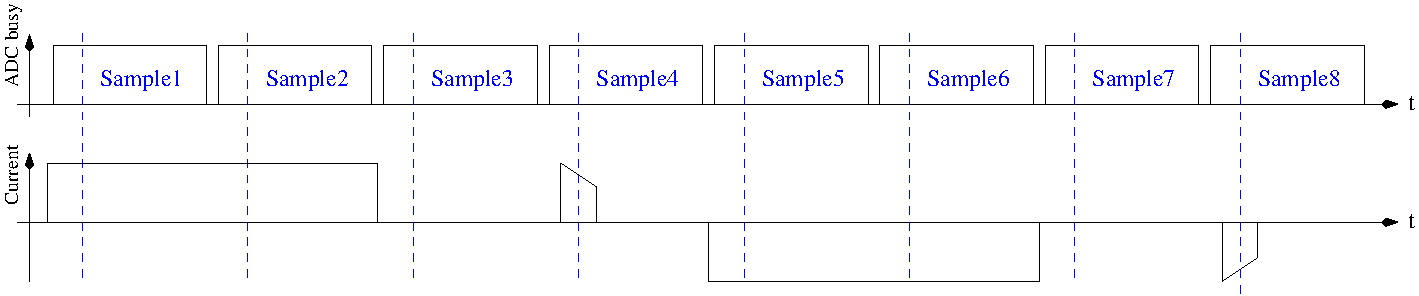
\includegraphics[width=18cm]{../FIG/Cap_esr2_timing.pdf}
  \caption{Časový průběh jednoho měřicího cyklu nového měření ESR}
  \label{fig:Cap_esr2_timing}
\end{figure}

\begin{figure}[H]
 \centering
 \begin{overpic}[width=15cm]{../FIG/Cap_esr2.pdf}
  \color{black}  
  \put(20,98){\makebox(0,0)[cb]{přední referenční měření}} 
  \put(20,72){\makebox(0,0)[cb]{přední referenční měření s pokusovým proudem}}
  \put(20,47){\makebox(0,0)[cb]{zpětné referenční měření}} 
  \put(20,21){\makebox(0,0)[cb]{zpětné referenční měření s pokusovým proudem }}      
 \end{overpic}
\vspace{-0,2cm} 
  \caption{Zjednodušené ESR měření kondenzátoru}
  \label{fig:Cap_esr2}
\end{figure}


Kratší nabíjecí impuls nejen umožňuje, aby měřená hodnota ESR byla měřena nižšími kapacitními hodnotami, ale může být také použita pro měření malých hodnot odporů pokud nemají měřitelnou indukčnost.

Tím  lze snížit rozlišení na hodnotách odporů pod \(10\Omega\) na \(0,01\Omega\).\\
Kromě toho lze zjistit nulový odpor jak pro měření odporů, tak i pro měření ESR v samočinné větvi kalibrace pro všechny tři kombinace testovacích pinů.

Pro stabilní výsledky by měl být dán pozor na pevnost spojů nebo svorky.\\
Doba měření trvá asi \(900\mu s\), což odpovídá frekvenci asi \(1,1kHz\).

Kvůli nedostatku nabíjecích impulzů je výsledek spíše jako měření s \(10kHz\).\\
Jako příklad je uveden na obrázku~\ref{pic:NewEsr10} měření \(10\mu F\) fólie kondenzátoru, jednou přímo a jednou se sériově připojeným\(2,7\Omega\) odporem.

Při srovnání obou diagramů můžete zřetelně vidět vliv dodatečného odporu.\\
Zde je také pochopitelné, proč měření ADC musí být uprostřed nabíjecího impulsu.\\
U velkých kondenzátorů zůstává nabíjecí proud kondenzátoru poměrně dobře konstantní,
aby se dalo měřit v časovém středu nabíjecího pulzu také průměrné napětí.

Pro malé kondenzátory je zde jasnější rozdíl, který je možné, pomocí známé kapacity, relativně dobře kompenzovat.

\begin{figure}[H]
  \begin{subfigure}[b]{9cm}
    \centering
    \includegraphics[width=9cm]{../PNG/NewEsr10uF0R0.png}
    \caption{bez sériového odporu}
  \end{subfigure}
  ~
  \begin{subfigure}[b]{9cm}
    \centering
    \includegraphics[width=9cm]{../PNG/NewEsr10uF2R7.png}
    \caption{s \(2,7\Omega\) sériovým odporem}
  \end{subfigure}
  \caption{Napětí \(10\mu F\)  kondenzátoru během nového měření ESR}
  \label{pic:NewEsr10}
\end{figure}

Při použití \(27\mu s\) dlouhých proudových impulzů, může být ESR kondenzátorů určeno od přibližně \(180nF\).

Aby šlo měřit i menší kondenzátory, byl současný puls ve verzi 1.11k dále redukován na \(8\mu s\).\\

Obrázky~\ref{pic:NewEsr2} ukazují křivku napětí na \(2,2\mu F\) kondenzátoru jednou bez a jednou se sériově připojeným \(2,7\Omega\) odporem.

\begin{figure}[H]
  \begin{subfigure}[b]{9cm}
    \centering
    \includegraphics[width=9cm]{../PNG/NewEsr2u2F0R0.png}
    \caption{bez sériového odporu}
  \end{subfigure}
  ~
  \begin{subfigure}[b]{9cm}
    \centering
    \includegraphics[width=9cm]{../PNG/NewEsr2u2F2R7.png}
    \caption{s \(2,7\Omega\) sériovým odporem}
  \end{subfigure}
  \caption{Křivka napětí \(2,2\mu F\) kondenzátoru během měření ESR s \(8\mu s\) nabíjecími impulsy}
  \label{pic:NewEsr2}
\end{figure}

Protože v diagramech \ref{pic:NewEsr2} nená okamžik převzetí napětí ADC rozpoznatelný,
je tento impuls roztaženě načten v obrázcích \ref{pic:NewEsr2zoom}.\\ Doba převzetí napětí
ADC je tady asi uprostřed obrazu.

\begin{figure}[H]
  \begin{subfigure}[b]{9cm}
    \centering
    \includegraphics[width=9cm]{../PNG/NewEsr2u2F0R0zoom.png}
    \caption{bez sériového odporu}
  \end{subfigure}
  ~
  \begin{subfigure}[b]{9cm}
    \centering
    \includegraphics[width=9cm]{../PNG/NewEsr2u2F2R7zoom.png}
    \caption{s \(2,7\Omega\) sériovým odporem}
  \end{subfigure}
  \caption{Výňatek z křivky napětí \(2,2\mu F\) kondenzátoru během měření ESR s \(8\mu s\) impulsy}
  \label{pic:NewEsr2zoom}
\end{figure}
 

Výsledky měření nové metody měření ESR jsou uvedeny na obrázku~\ref{fig:Cesr2}.\\
Hodnoty ESR se liší od výsledků na obrázku~\ref{fig:Cesr} kvůli závislosti na frekvenci.\\
Porovnávací hodnoty  LCR-měřiče byly stanoveny na \(10kHz\).

\begin{figure}[H]
\centering
 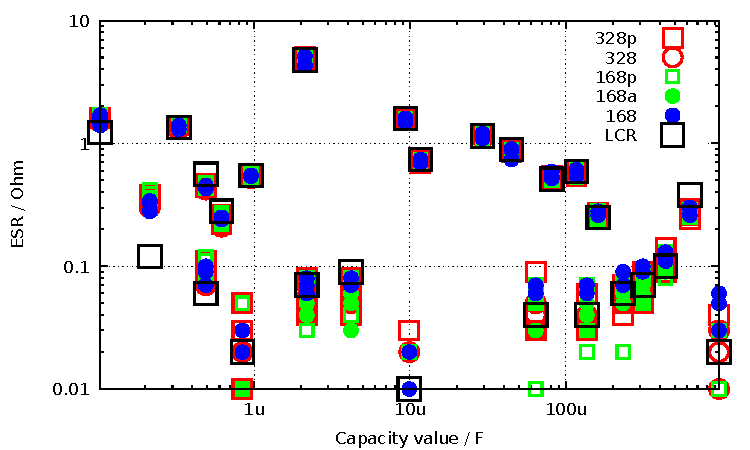
\includegraphics[width=16cm]{../GNU/Cesr2.pdf}
\caption{Výsledky měření měření ESR s 15 různými ATmega, 2 metodou}
\label{fig:Cesr2}
\end{figure}

Série měření s elektrolytickými kondenzátory různých velikostí je uvedena na obrázku \ref{fig:ElcoESR}.\\
Zobrazuje výsledky měřicího přístroje PeakTech 3315 LCR při různých frekvencích měření a
výsledky porovnání tranzistoru.

Hodnoty odporů jsou v tomto diagramu zobrazeny logaritmicky.\\
Ve všech případech leží výsledky testeru blízko výsledků LCR-měřidla při \(10kHz\) frekvenci měření.\\ 
Pouze \(500\mu F/3V\) kondenzátor byl starší, všechny ostatní byly nové.

\begin{figure}[H]
\centering
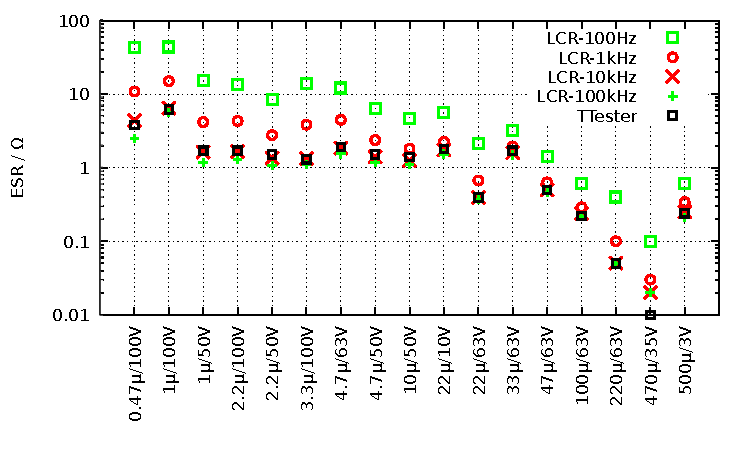
\includegraphics[width=18cm]{../GNU/Elco_esr.pdf}
\caption{Výsledky ESR měření různých elektrolytických kondenzátorů}
\label{fig:ElcoESR}
\end{figure}

Vzhledem k tomu, že lze s novou metodou také měřit odpory, jsou na obr.~\ref{fig:res_esr} měření chyby při měření několika odporů pod \(10\Omega\) , každý s třemi exempláři, na různých ATmega zobrazeny.  

\begin{figure}[H]
\centering
\includegraphics[width=18cm]{../GNU/res_esrCZ.pdf}
\caption{Chyba měření u odporů, měřením ESR}
\label{fig:res_esr}
\end{figure}

Od softwarové verze 1.12k byla délka nabíjecího impulsu pro kondenzátory zkrácena na \(2\mu s\), aby bylo možné měření ESR hodnoty ESR i u menších hodnot kapacity.

Nyní je možné měřit hodnotu ESR od kapacity \(20nF\).\\
S klesající kapacitou se chyba měření zvyšuje. Důvodem je klesající časová konstanta RC obvodu, která je u \(20nF\) je pouze asi \(14.4\mu s\).

V důsledku toho se mění významně napětí během \(2\mu s\) proudového impulsu.\\
Software může zvolit čas odběru vzorků pouze přesně na jeden takt procesoru. Ale vstupní filtr
ADC má časovou konstantu asi \(0.24\mu s\), která se bohužel od exempláře k exempláři trochu liší.

Na toto změnu časové konstanty filtru nelze brát v programu ohled.
Pro tento účel by musela být doba odebírání ADC nastavena přesně na zlomek doby taktu procesoru.

S rostoucími hodnotami kapacity měřeného objektu se zvyšuje časová konstanta a změna napětí během nabíjecího impulzu se snižuje.

Změna časové konstanty vstupního filtru ADC má tedy menší a menší vliv na výsledky měření.\\
Příklady na obrázku~\ref{pic:Cesr_22n} ukazují výsledky 10 různých zkoušečů.

Na levé straně byly měřeny kondenzátory s vyššími hodnotami ESR. Výsledek vypadá ve srovnání s výsledkem měření měřícího přístroje Peaktech 2170 LCR u \(10kHz\) a \(100kHz\) uspokojivé.

Na pravé straně jsou zobrazeny naměřené hodnoty kvalitních kondenzátorů s nízkými hodnotami ESR.
I když je limit postupu jasně viditelný, je výsledek stále lepší než vůbec žádná informace.

V každém případě je možné odhadnout kvalitu kondenzátoru i při nízké kapacitě.

\begin{figure}[H]
  \begin{subfigure}[b]{9cm}
    \centering
    \includegraphics[width=9cm]{../GNU/Cesr_22nCZ.pdf}
    \caption{vyšší ESR hodnoty}
  \end{subfigure}
  ~
  \begin{subfigure}[b]{9cm}
    \centering
    \includegraphics[width=9cm]{../GNU/Cesr_22n_lowCZ.pdf}
    \caption{nižší ESR hodnoty}
  \end{subfigure}
  \caption{ESR měření kondenzátorů s nízkou kapacitou}
  \label{pic:Cesr_22n}
\end{figure}
 
U procesorů s pamětí s kapacitou více než 16 kB bude od softwarové verze 1.12k použito, pro polovinu jednotlivých měření, kromě \(680\Omega\) odporu, ještě paralelně připojený \(470k\Omega\) odpor
k možnosti změny měřicího proudu.

Bohužel je dodatečný proud velmi nízký, takže zvýšení napětí dosáhne jen malé změny výsledku ADC.
Zvýšení napětí představuje pouze asi 20\% jednoho ADC bitu s interní \(1.1V\) referencí.

Bylo by žádoucí, aby na ADC vstupu bylo malé šumící napětí, které by změnilo individuální hodnoty ADC.
To by pak umožnilo statistické zvýšení rozlišení ADC pomocí zprůměrování. 


\subsection{Ztráta napětí po nabíjecím impulsu, Vloss}
Při metodě měření velkých kapacit se zkoumá ztráta napětí po nabíjecím impulzu v deaktivovaném stavu.

U elektrolytických kondenzátorů, se po krátké době, nabíjecí napětí opět mírně sníží.\\
Tato ztráta napětí může být způsobena paralelně zapojeným odporem.

Předpokládám, že ztráta napětí v elektrolytických kondenzátorech kvůli internímu rozdělení náboje způsobené nabíjecím impulsem.

Při pomalém nabíjení, jak je to provedeno  u menších kapacit s \(470k\Omega\)  odporem
je toto přerozdělení dokončeno již během procesu nabíjení.\\ Pak nedochází k žádné měřitelné ztrátě napětí
poplatku v daném časovém období.

Bude-li stejný elektrolytický kondenzátor, ale krátkými pulzními impulsy proudu nabíjen, je také zde i ztráta napětí způsobená následným přerozdělením pozorovatelná.

Stejný účinek je v menší míře pozorován u keramických kondenzátorů.\\
Podle předchozích pozorování jsou kondenzátory s několika  \% ztráty napětí podezřelé.

Obzvláště poznatelné z hlediska ztráty napětí jsou starší papírové kondenzátory, které jsou výzvou í pro jiné měřicí přístroje. 

Chtěl bych to objasnit v následující tabulce.

\vspace{0.5 cm}

\begin{tabular}{| l | c | c | c | c | c | c |}
   \hline
Kondenzátor & kapacita      & PeakTech     & Voltcraft & PeakTech & tester \\
Typ        &   & LCR 2170     & M2650-B   &  3315    &       \\
    \hline
    \hline
Papír     & 4700pF      & 6.75-10.36nF & 8.00nF    &  25.40nF &  10.71nF   \\
           &             &  Q=2.5-32    &           &          &  Vloss=11 \% \\
    \hline
Papír     & 6800pF      & 9.40-11.40nF & 10.41nF   &  23.30nF &  11.65nF  \\
           &             &  Q=5-25      &           &          &  Vloss=5.0 \% \\
    \hline
neznámý  & 4700pF      & 5.85-6.33nF  & 6.12nF    &  6.90nF  &  6225pF  \\
           &             &  Q=16-87     &           &          &  Vloss=1.7 \% \\
    \hline
Folie      & 7870pF      & 7.86-7.87nF  & 7.95nF    &  7.95nF  &  7872pF  \\
           &             &  Q= \textgreater~1540    &           &          &  Vloss=0 \% \\
    \hline
Papír     & 22000pF     & 37.4-57.5nF  & 52.8nF    &  112nF   &  118.5nF \\
           &             &  Q=2.5-32    &           &          &  Vloss=12 \% \\
    \hline
Folie      & 22600pF     & 22.4-22.5nF  & 22.57nF   & 22.69nF  &  22.54nF \\
           &             & Q= \textgreater~1540     &           &          &  Vloss=0 \% \\
    \hline
Papír     & 100nF       & 144-256nF    & 177nF     &  318nF   &  529.7nF \\
           &             & Q=2.6-28     &           &          &  Vloss=12 \% \\
    \hline
Keramika  & 100nF       & 97.7-102nF   & 103.7nF   & 103.3nF  &  103.1nF \\
           &             & Q=90-134     &           &          &  Vloss=0.1 \% \\
    \hline
Folie      & 100nF       & 98.0-101nF   & 101.4nF   & 102.2nF  &  101.6nF \\
           &             & Q=58-700     &           &          &  Vloss=0 \% \\
    \hline
\end{tabular}
\vspace{0.5 cm}


V tabulce je vidět, že je kapacita všech kondenzátorů s fólií určena všemi měřicími přístroji s uspokojivou přesností.

Kapacity a Q hodnocení měřidla PeakTech LCR jsou minimální a maximální výsledky měření v kmitočtovém
rozsahu od \(100Hz\) do \(100kHz\).

Ve všech příkladech v tabulce je ztráta napětí Vloss testeru velká, pokud mají kondenzátory nízkou kvalitu.

Pouze v tomto případě existují i velké odchylky při sledování měřené kapacity.\\
Takže ztráty napětí kondenzátoru lze testerem měřit, pokud je měřená kapacita větší než \(5000pF\).

\subsection{Samostatné měření kapacity a ESR}
Samostatné měření kapacity s následným měřením ESR je pouze pro ATmega s dostatečnou pamětí
volitelné pomocí dialogového menu. Tento typ měření je určen k měření kondenzátorů v obvodech v zapájeném stavu.\\
Ujistěte se před začátkem měření, že jsou všechny kondenzátory na desce s plošnými spoji vybity. 
Aby bylo možné měřit v těchto obvodech, je zajištěno, že je měřicí napětí, jen nepatrně nad \(300mV\).
Kromě toho je měření provedeno pouze s \(680\Omega\) odporem, k zmírnění vlivu zbytkových proudů připojených součástek na obvodové desce.
Aby bylo možné měřit nejmenší možné kapacitní hodnoty, je začínající nabíjecí impulz pouze \(200\mu s\) krátký. Pokud lze z nabíjejícího napětí očekávat, že i při dlouhém \(2ms\) nabíjecím impulsu, nabíjecí napětí
nepřekročí \(300mV\), bude nadále nabíjeno \(2ms\). Pokud, při velkých kapacitách, není přesto žádné významné zvýšení napětí pozorováno, bude pokračováno dokonce s \(20ms\) dlouhými nabíjejícími impulsy. Když se  napětí přiblíží k \(300mV\), vrátí se program zpět ke kratším nabíjecím impulsům. Celková nabíjecí doba bude sečtena a poté co bude \(300mV\) napěťová hranice překročena bude kapacita určena z nabitého napětí a doby nabíjení.
S touto metodou je možné, měřit kapacitu něco pod \(2\mu F\). Horní mez kapacity při tomto měření,
v důsledku časového limitu nabíjení na \(2,5s\), je asi \(50mF\).
Po změření hodnoty kapacity, bude hodnota ESR měřena s již uvedenou metodou v sekci~\ref{sec:ESR2}.
Výsledky jsou zobrazeny jen krátce a pak se okamžitě začne s dalším měřením.
Série měření se přeruší po 250 měřeních, nebo stisknutím tlačítka.

Poté se tester vrátí k provoznímu menu.

\subsection{Výsledky měření kondenzátorů}
Výsledky mých měření jsou uvedeny na obrázku~\ref{fig:mega8cap} pro tři ATmega8.\\
Kromě toho existují některé hodnoty původního softwaru s korekčním faktorem
od 0,88~(\(-12\%\)).
Další výsledky verzí ATmega8 jsou zobrazeny na obrázcích~\ref{fig:mega8Acap} a \ref{fig:mega8Lcap}.

Výsledky měření stejných kondenzátorů s ATmega168 jsou uvedeny na obrázku~\ref{fig:mega168cap}.\\
Referencí na výpočet chyb jsou výsledky měření měřidla PeakTech 2170 LCR, nikoliv tiskové hodnoty součástí.

Větší relativní chyby měření s velkými kondenzátory jsou částečně způsobeny vysokou měřicí
frekvencí (\(100Hz\)) měřícího  LCR přístroje pro velké elektrolytické kondenzátory, na druhé straně, hraje  roli, špatná kvalita elektrolytických kondenzátorů.

\begin{figure}[H]
\centering
\includegraphics[width=18cm]{../GNU/Mega8capCZ.pdf}
\caption{Procentní chyba měření kondenzátoru se třemi ATmega8}
\label{fig:mega8cap}
\end{figure}

\begin{figure}[H]
  \begin{subfigure}[b]{9cm}
    \centering
    \includegraphics[width=9cm]{../GNU/Mega8AcapCZ.pdf}
    \caption{se třemi ATmega8A}
    \label{fig:mega8Acap}
  \end{subfigure}
  ~
  \begin{subfigure}[b]{9cm}
    \centering
    \includegraphics[width=9cm]{../GNU/Mega8LcapCZ.pdf}
	  \resizebox{9cm}{!}{\includegraphics[]{../GNU/Mega8LcapCZ}}
    \caption{se třemi ATmega8L}
    \label{fig:mega8Lcap}
  \end{subfigure}
  \caption{Procentální chyba měření kondenzátorů}
\end{figure}

\begin{figure}[H]
\centering
\includegraphics[width=18cm]{../GNU/Mega168capCZ.pdf}
\caption{Procentuální chyba měření kondenzátorů se třemi ATmega168}
\label{fig:mega168cap}
\end{figure}

Jak je obtížné najít správnou referenční hodnotu pro měření kondenzátoru, je znázorněno na obrázku~\ref{fig:capcompare}.\\
Jako reference se zde nejlépe odhaduje. Křivka ,,Multimeter'' zobrazuje odchylky, které mají a
Peaktech ~ 3315 multimetru.\\
Další křivka ,,LCR'' zobrazuje odchylky naměřené měřičem Peaktech ~ 2170 LCR v nejpříznivějším kmitočtovém rozsahu.
Pro srovnání, křivka ,,ATmega168as'' také ukazuje odchylky měření testeru vybaveného ATmega168.\\
Zda jsou zobrazeny chyby, ale skutečné chyby měření příslušného zařízení, musíme pochybovat, stejně jako
odhad velikosti kapacity neodpovídá skutečné kapacitě.

\begin{figure}[H]
\centering
\includegraphics[width=18cm]{../GNU/capcompareCZ.pdf}
\caption{Porovnání měření kondenzátoru s multimetrem, měřičem LCR a ATmega168}
\label{fig:capcompare}
\end{figure}

Odchylky měření jsou výsledkem tří různých ATmega168, které jsou uvedeny na obrázku~\ref{fig:mega168all}.
Zde byl LCR-měřič jako základ pro srovnání měření.

V důsledku toho výsledky měření tří různých ATmega168A na obrázku~\ref{fig:mega168Aall}, 
tří různých ATmega168PA na obrázku~\ref{fig:mega168PAall}  a tří různých
ATmega328 na obrázku~\ref{fig:mega328all} stejně jako tři ATmega328P na obrázku~\ref{fig:mega328Pall}.

V úvahu byla vzata pouze nulová hodnota měření kapacity \(39pF\), všechny ostatní možnosti korekce se zde
nepoužívají.

Tato nulová hodnota již obsahuje \(2-3pF\), který je způsoben přibližně \(12cm\) dlouhými připojovacími kabely s krokosvorkami.

Návrh desky plošných spojů DPS také ovlivňuje tuto nulovou hodnotu.\\ Tuto nulovou hodnotu jsem zjistil při použití verze desky ,,DG2BRS V 5.2.1''.

\begin{figure}[H]
  \begin{subfigure}[b]{9cm}
    \centering
    \includegraphics[width=9cm]{../GNU/Mega168allCZ.pdf}
    \caption{tři ATmega168}
    \label{fig:mega168all}
  \end{subfigure}
  ~
  \begin{subfigure}[b]{9cm}
    \centering
    \includegraphics[width=9cm]{../GNU/Mega168AallCZ.pdf}
    \caption{tři ATmega168A}
    \label{fig:mega168Aall}
  \end{subfigure}
  \caption{Chyba měření kondenzátoru, nekalibrovaná}
\end{figure}

\begin{figure}[H]
\centering
\includegraphics[width=16cm]{../GNU/Mega168PAallCZ.pdf}
\caption{Chyba měření kondenzátoru třemi ATmega168PA, nekalibrovaná}
\label{fig:mega168PAall}
\end{figure}

\begin{figure}[H]
  \begin{subfigure}[b]{9cm}
    \centering
    \includegraphics[width=9cm]{../GNU/Mega328allCZ.pdf}
    \caption{tři ATmega328}
    \label{fig:mega328all}
  \end{subfigure}
  ~
  \begin{subfigure}[b]{9cm}
    \centering
    \includegraphics[width=9cm]{../GNU/Mega328PallCZ.pdf}
    \caption{tři ATmega328P}
    \label{fig:mega328Pall}
  \end{subfigure}
  \caption{Chyba měření kondenzátoru nekalibrovaná}
\end{figure}

Pro dosažení nejlepší přesnosti měření musí software odpovídat individuálním vlastnostem použitého ATmega.

Pro tento účel může být použito korekční napětí REF\_C\_KORR, které se používá pro měření malých kapacit.

Opravné napětí \(1mV\) vede ke snížení indikátoru kapacity o \(0,11\%\).\\
Při automatickém nastavení je REF\_C\_KORR pouze ofset k naměřenému diferenčnímu napětí nabitého kondenzátoru
a interní referenci.

U velkých kapacit lze zadat hodnotu percentilu C\_H\_KORR o kterou jsou výsledky měření velké.\\
Vzhledem k tomu, že velké kondenzátory jsou většinou nekvalitní elektrolytické kondenzátory, je zjištění
skutečné hodnoty kapacity, a tím také určení chyby měření, zde obzvláště obtížné.

Zejména s ATmega168 jsem pozoroval chybu měření s malými kapacitními hodnotami,
což závisí na rychlosti nabití nabíjecího napětí.

Obrázek~\ref{fig:mega168optcap}  ukazuje chybu měření v případě měření kondenzátoru pouze s uvážením
nulové hodnoty (168-3-A), přičemž korekční faktor pro malé kapacity REF\_C\_KORR=66 a korekční faktor pro velké
Kondenzátory C\_H\_KORR=5 (168-3-B), a dále jako křivka 168-3-C s ohledem na vzrůst napětí (COMP\_SLEW1=4000 a COMP\_SLEW2=220) a vlastním vybíjecím chováním velkých kondenzátorů.

Faktor vzrůstu napětí lze vypočítat podle \(\frac{COMP\_SLEW1}{cval+COMP\_SLEW2} - \frac{COMP\_SLEW1}{COMP\_SLEW2}\), při čemž je cval změřená kapacita v pF.

\begin{figure}[H]
\centering
\includegraphics[width=16cm]{../GNU/Mega168cap_optCZ.pdf}
\caption{Optimalizace měření kondenzátorů ATmega168}
\label{fig:mega168optcap}
\end{figure}

\subsection{Automatické nastavení měření kondenzátorů}

Automatické nastavení se skládá ze dvou částí.

První částí je nastavení nulové rovnováhy měření kondenzátoru.
K tomuto účelu se průměrná hodnota naměřené kapacity určuje v rutině automatického testování, když není kondenzátor připojen.
Průměrné hodnoty jsou stanoveny z 8 měření u všech 6 kombinací měření.

Po úspěšném nastavení jsou korekční hodnoty zaznamenávány v paměti EEPROM a používány pro budoucí měření.

Složitější je eliminace rozptylu vzorku při měření kondenzátorů na přibližně \(40\mu F\), jak bylo zobrazeno na obrázcích \ref{fig:mega168all}, \ref{fig:mega168Aall} a \ref{fig:mega168PAall}.\\
Hlavní příčinou bylo zjištěno odlišné chování (offset napětí) analogového komparátoru.

Na obrázku \ref{fig:CompAdjust} jsou zobrazena data z devíti zkoumaných procesorů.\\
Body ,,diff2ref'' ukazují rozdíl napětí, který vznikne po nabíjení kondenzátoru s \(660nF\) na
příslušném vnitřním referenčním napětí.

V ideálním případě by toto napětí bylo vždy nulové, pokud by analogový komparátor dal včasný signál k ukončení nabíjecího procesu.

Krátký čas  ATmega administrace by neměl vést, při relativně velké kapacitě, k měřitelnému zvýšení napětí.

Z obrázků \ref{fig:mega168all}, \ref{fig:mega168Aall} a \ref{fig:mega168PAall} ukazují body ,,CapErr'' 
odhadované chyby měření jednotlivých vzorků ATmega v promile.

Je nápadné, jak se body ,,CapErr'' řídí body ,,diff2ref''.
Proto body ,,diff''  ukazují rozdíl mezi příslušnými body ,,CapErr'' a ,,diff2ref''.

Při střední hodnotě pro ,,diff'' lze tedy udělat dobrý odhad korekce měření kondenzátoru z rozdílu napětí kondenzátoru po nabití k vnitřnímu referenčnímu napětí vypočítat.

Takže v druhé části kalibračního postupu musí být mezi pinem 1 a 3 připojen vysoce kvalitní kondenzátor
s kapacitou mezi \(100nF\) und \(20\mu F\).
 
Měl by to být fóliový kondenzátor, pokud možno žádný keramický kondenzátor a rozhodně ne
elektrolytický kondenzátor.

Pro toto srovnání nemusí být hodnota kapacity  přesně známa.

\begin{figure}[H]
\centering
\includegraphics[]{../GNU/ComparatorAdjustCZ.pdf}
\caption{Data od devíti ATmega168 procesorů}
\label{fig:CompAdjust}
\end{figure}

Grafy \ref{fig:mega168cal}, \ref{fig:mega168Acal}, \ref{fig:mega168PAcal},  \ref{fig:mega328cal} a
\ref{fig:mega328Pcal} zobrazují výsledky měření stejnými procesory ve standardní konfiguraci softwaru po automatické kalibraci.

Všechny procesory byly naprogramovány se stejným softwarem, pouze volba Makefile ,,PARTNO = '' musela být, vzhledem k AVRDUDE programu, upravena na jiný typ procesoru (,,m168'', ,,m168p'', ,,m328'' nebo ,,m328p'') upravena.

Po programování byl s každým ATmega spuštěn Autotest a při Test~10, připojen na piny~1 a~3 \(330nF\) kondenzátor.

\begin{figure}[H]
  \begin{subfigure}[b]{9cm}
    \centering
    \includegraphics[width=9cm]{../GNU/Mega168calCZ.pdf}
    \caption{tři ATmega168}
    \label{fig:mega168cal}
  \end{subfigure}
  ~
  \begin{subfigure}[b]{9cm}
    \centering
    \includegraphics[width=9cm]{../GNU/Mega168AcalCZ.pdf}
    \caption{tři ATmega168A}
    \label{fig:mega168Acal}
  \end{subfigure}
  \caption{Chyba měření kondenzátorů, po kalibraci}
\end{figure}

\begin{figure}[H]
\centering
\includegraphics[width=16cm]{../GNU/Mega168PAcalCZ.pdf}
\caption{Chyba měření kondenzátorů u tří ATmega168PA, po kalibraci}
\label{fig:mega168PAcal}
\end{figure}

\begin{figure}[H]
  \begin{subfigure}[b]{9cm}
    \centering
    \includegraphics[width=9cm]{../GNU/Mega328calCZ.pdf}
    \caption{tři ATmega328}
    \label{fig:mega328cal}
  \end{subfigure}
  ~
  \begin{subfigure}[b]{9cm}
    \centering
    \includegraphics[width=9cm]{../GNU/Mega328PcalCZ.pdf}
    \caption{tři ATmega328P}
    \label{fig:mega328Pcal}
  \end{subfigure}
  \caption{Chyba měření kondenzátorů, po kalibraci}
\end{figure}

Ke konci chci vyjasnit efekt možnosti AUTO\_CAL v autotestu.\\
Následující diagram \ref{fig:MegaAuto} ukazuje, ještě jednou, výsledky tří ATmega procesorů
s největší měřící odchylkou před a po kalibraci.

Body s koncovým znakem ,,unc'' zobrazují odchylky bez kalibrace.\\
Řádky končící na ,,cal'' ukazují odchylky stejných procesorů
se stejným softwarem po kalibraci v režimu automatického testování.

Příčina odchylek měření u velkých kondenzátorů (\textgreater\(40\mu F\))  je
zatím neznámá.\\ Všechny kondenzátory používané pro tuto řadu měření byly
fóliové nebo keramické kondenzátory s hodnotou (\(56pF\), \(100pF\) a \(3,3nF\)), žádné elektrolytické kondenzátory.

\begin{figure}[H]
\centering
\includegraphics[width=16cm]{../GNU/MegaAutoCZ.pdf}
\caption{Chyba měření kapacity tří ATmega před a po kalibraci}
\label{fig:MegaAuto}
\end{figure}

Obvod s ATmega644 nebo ATmega1284 předpokládá na desce pro kalibraci kondenzátor.\\
Schéma \ref{fig:Mega1284} zobrazuje výsledky měření kondenzátorů s ATmega1284,
jak s \(100nF\)  keramickým kondenzátorem kalibrován na desce (1284-int) tak i s externím foliovém \(220nF\) kondenzátorem,\\
ve srovnání s výsledky ATmega328 na jiné desce.

\begin{figure}[H]
\centering
\includegraphics[width=16cm]{../GNU/Mega1284CZ.pdf}
\caption{Chyba měření kondenzátorů s ATmega1284 v porovnání s ATmega328}
\label{fig:Mega1284}
\end{figure}
